%%%%%%%%%%%%%%%%%%%%%%%%%%%%%%%%%%%%%%%%%%%%%%%%%%%%%%%%%%%%%%%%%%%%%
%% This is a (brief) model paper using the achemso class
%% The document class accepts keyval options, which should include
%% the target journal and optionally the manuscript type.
%%%%%%%%%%%%%%%%%%%%%%%%%%%%%%%%%%%%%%%%%%%%%%%%%%%%%%%%%%%%%%%%%%%%%
\documentclass[journal=jacsat,manuscript=article]{achemso}

%%%%%%%%%%%%%%%%%%%%%%%%%%%%%%%%%%%%%%%%%%%%%%%%%%%%%%%%%%%%%%%%%%%%%
%% Place any additional packages needed here.  Only include packages
%% which are essential, to avoid problems later. Do NOT use any
%% packages which require e-TeX (for example etoolbox): the e-TeX
%% extensions are not currently available on the ACS conversion
%% servers.
%%%%%%%%%%%%%%%%%%%%%%%%%%%%%%%%%%%%%%%%%%%%%%%%%%%%%%%%%%%%%%%%%%%%%
\usepackage[version=3]{mhchem} % Formula subscripts using \ce{}
\usepackage{amsmath}
\usepackage{subcaption}

%%%%%%%%%%%%%%%%%%%%%%%%%%%%%%%%%%%%%%%%%%%%%%%%%%%%%%%%%%%%%%%%%%%%%
%% If issues arise when submitting your manuscript, you may want to
%% un-comment the next line.  This provides information on the
%% version of every file you have used.
%%%%%%%%%%%%%%%%%%%%%%%%%%%%%%%%%%%%%%%%%%%%%%%%%%%%%%%%%%%%%%%%%%%%%
%%\listfiles

%%%%%%%%%%%%%%%%%%%%%%%%%%%%%%%%%%%%%%%%%%%%%%%%%%%%%%%%%%%%%%%%%%%%%
%% Place any additional macros here.  Please use \newcommand* where
%% possible, and avoid layout-changing macros (which are not used
%% when typesetting).
%%%%%%%%%%%%%%%%%%%%%%%%%%%%%%%%%%%%%%%%%%%%%%%%%%%%%%%%%%%%%%%%%%%%%
\newcommand*\mycommand[1]{\texttt{\emph{#1}}}

%%%%%%%%%%%%%%%%%%%%%%%%%%%%%%%%%%%%%%%%%%%%%%%%%%%%%%%%%%%%%%%%%%%%%
%% Meta-data block
%% ---------------
%% Each author should be given as a separate \author command.
%%
%% Corresponding authors should have an e-mail given after the author
%% name as an \email command. Phone and fax numbers can be given
%% using \phone and \fax, respectively; this information is optional.
%%
%% The affiliation of authors is given after the authors; each
%% \affiliation command applies to all preceding authors not already
%% assigned an affiliation.
%%
%% The affiliation takes an option argument for the short name.  This
%% will typically be something like "University of Somewhere".
%%
%% The \altaffiliation macro should be used for new address, etc.
%% On the other hand, \alsoaffiliation is used on a per author basis
%% when authors are associated with multiple institutions.
%%%%%%%%%%%%%%%%%%%%%%%%%%%%%%%%%%%%%%%%%%%%%%%%%%%%%%%%%%%%%%%%%%%%%
\author{Elliott Capek}
\affiliation{Department of Biochemistry, Oregon State University}
\email{capeke@oregonstate.edu}
\phone{(971) 207 8193}
\author{Hassan Alnatah}
\author{Laikana Ly}
\author{Joey Orton}
%% \alsoaffiliation[]{}
\author{Aidan Estelle}
%% \affiliation{Department of Biochemistry, Oregon State University}

%%%%%%%%%%%%%%%%%%%%%%%%%%%%%%%%%%%%%%%%%%%%%%%%%%%%%%%%%%%%%%%%%%%%%
%% The document title should be given as usual. Some journals require
%% a running title from the author: this should be supplied as an
%% optional argument to \title.
%%%%%%%%%%%%%%%%%%%%%%%%%%%%%%%%%%%%%%%%%%%%%%%%%%%%%%%%%%%%%%%%%%%%%
\title[]{Click chemistry reveals an alternate mechanism for HPII catalase}

%%%%%%%%%%%%%%%%%%%%%%%%%%%%%%%%%%%%%%%%%%%%%%%%%%%%%%%%%%%%%%%%%%%%%
%% Some journals require a list of abbreviations or keywords to be
%% supplied. These should be set up here, and will be printed after
%% the title and author information, if needed.
%%%%%%%%%%%%%%%%%%%%%%%%%%%%%%%%%%%%%%%%%%%%%%%%%%%%%%%%%%%%%%%%%%%%%
\keywords{Catalase, noncanonical amino acid, active site, channel flow}

\begin{document}
%%%%%%%%%%%%%%%%%%%%%%%%%%%%%%%%%%%%%%%%%%%%%%%%%%%%%%%%%%%%%%%%%%%%%
%% The manuscript does not need to include \maketitle, which is
%% executed automatically.  The document should begin with an
%% abstract, if appropriate.  If one is given and should not be, the
%% contents will be gobbled.
%%%%%%%%%%%%%%%%%%%%%%%%%%%%%%%%%%%%%%%%%%%%%%%%%%%%%%%%%%%%%%%%%%%%%
\begin{abstract}
  %% This is an example document for the \textsf{achemso} document
  %% class, intended for submissions to the American Chemical Society
  %% for publication. The class is based on the standard \LaTeXe\
  %% \textsf{report} file, and does not seek to reproduce the appearance
  %% of a published paper.

  %% This is an abstract for the \textsf{achemso} document class
  %% demonstration document.  An abstract is only allowed for certain
  %% manuscript types.  The selection of \texttt{journal} and
  %% \texttt{manuscript} will determine if an abstract is valid.  If
  %% not, the class will issue an appropriate error.
  Abstract abstract abstracts abstract. Abstract abstract abstracts abstract. Abstract abstract abstracts abstract. Abstract abstract abstracts abstract. Abstract abstract abstracts abstract. Abstract abstract abstracts abstract. Abstract abstract abstracts abstract. Abstract abstract abstracts abstract.\\
\end{abstract}

%%%%%%%%%%%%%%%%%%%%%%%%%%%%%%%%%%%%%%%%%%%%%%%%%%%%%%%%%%%%%%%%%%%%%
%% Start the main part of the manuscript here.
%%%%%%%%%%%%%%%%%%%%%%%%%%%%%%%%%%%%%%%%%%%%%%%%%%%%%%%%%%%%%%%%%%%%%
\section{Introduction}
Catalase is an enzyme which catalyzes the breakdown of hydrogen peroxide into water and oxygen gas. This is an important detoxification reaction, since hydrogen peroxide is a reactive toxin generated by several biological processes. Catalase is a tetrameric protein which uses a heme group in its active site to facilitate the breakdown of hydrogen peroxide. The molecular mechaninism of catalase proceeds in two steps. First, the heme reduces a hydrogen peroxide, producing water and the so-called Cpd I. Then Cpd I oxidizes a second hydrogen peroxide, producing water and oxygen gas. This second step is mediated by a histidine near the active site \cite{alfonso-prieto}.

Catalase's activity is nearly diffusion-limited \cite{kcatkm, difflimit}. This rate suggests that nearly every step in the substrate-enzyme interaction is optimized for speed. Understanding the optimizations of diffusion-limited proteins can provide many insights into how proteins achieve their functions. Catalase has a variety of interesting quirks for funneling substrate into its active pocket. The enzyme has a number of high-H2O2-residency surface residues near its active channel, which are believed to concentrate the substrate near the entrance to the active channel \cite{concentrateh2o2}. The active channel itself seems optimized to maximize substrate flow, to the point that mutagenesis to open the channel decreases enzyme activity \cite{substrateflow}. The channel seems to be capable of selecting the molecules which enter it using a patch of hydrophobic residues which are situated to preferentially pass the bulkier H2O2 \cite{molecularruler}. Even the directionality of substrate within the channel seems to be controlled: one channel is used for substrate entrance, and the other for product exit \cite{lateralchannel}. An new finding suggests that catalase might control not just the presence of hydrogen peroxide, but even its orientation as it enters the active site. It is believed that an electric field from a negative Asn residue to the positive heme acts to orient the H2O2 dipole, positioning the molecule such that it enters the active site at an angle ideal for reacting \cite{electricpotential}. This use of an electric field over a long range to create an ``orienting field'' is a new and exciting usage of residues to achieve a function; understanding its role in catalase may help to understand the mechanisms of other proteins.

In this study we hope to study the proposed orienting field optimization and its influence on catalase activity. In particular, we hope to carefully disrupt the wildtype active site potential environment by introducing a new charged residue, then examine the effect this disruption has on activity. For meaningful results, we must be careful to not introduce structural modifications to the enzyme. To ensure this, we will use genetic code expansion to incorporate 3-nitrotyrosine in place of tyrosine 206. The T206NY mutation will add only 30 $\AA^3$ of steric bulk \cite{3ntsize}, so should have minimal influence on active site structure. The theorized results of this addition are diagrammed in Figure \ref{fig:hypothesis}. To study the influence of field disruption on activity, we will study the activity of T206NY above and below its pKa of 6.8 \cite{3ntsize}. Wildtype catalase activity is constant under pH values from 5 to 10 \cite{phdependence,kcatkm}, so pH-dependence should only be seen if electric environment in the active site is important for activity.\\

\begin{figure}
  \caption{Depiction of catalase active pocket. \textbf{Left:} wildtype pocket with proposed ligand-orienting E-field \cite{electricpotential}. The field should orient H2O2 for optimal reaction with the heme. \textbf{Right:} modified HPII-3NY with a deprotonated 3-nitrotyrosine residue at site 206, with hypothetical augmented E-field. The disrupted E-field should result in un- or mis-aligned substrate.}
  \label{fig:hypothesis}
\end{figure}

\section{Methods}
\textbf{Protein expression}\\
Wildtype protein was expressed by transforming the plasmid pBad-HPII (Addgene ID 105839), containing WT HPII gene, into competent \textit{E. coli} DH10B cells via heat-shock. pBad-HPII plasmid includes ampicillin resistance, an imidazole promoter, and a 6xHis tag on the N-term of the HPII gene. Cells were then grown in autoinduction media with an arabinose inducer (0.1\% aspartate pH 7.5, 0.2\% glycerol, 100$\mu g / mL$ ampicillin, mineral salts, 0.05\% glucose, 20mM MgSO4, 0.05\% arabinose, trace metals and AA mix) for 48 hours, shaking, at 37C. Cells were then pelletized and stored at -80C.\\

The same protocol was followed for the ncAA mutant catalases F206NY and F206pAzF, except protein plasmid pBad-HPII TAG206 (Addgene ID 105846) was used as a base. ncAA translation machinery plasmids pDule-3-nitrotyrosine (Addgene ID 85498) and pDule-pCNF (85494), which contain a tetracycline resistance gene, a TAG tRNA, and a compatible tRNA synthase, were co-transformed into DH10B along with pBAD-HPII TAG206 for respective F206NY and F206pAzF cell lines. ncAA autoinduction media was supplemented with $25\mu g / mL$ tetracycline to select for both plasmids.\\

OD600 measurements of cultures at 48h growth time were 0.65, 0.58 and 0.45 arb. units for WT, F206NY and F206pAzF cells.\\

\textbf{Protein purification}\\
Pelletized cells were reconstituted in TALON equilibration buffer (50mM sodium phosphate, 300mM NaCl) and microfluidized, also in equilibration buffer. Lysed cells were spun down at 15K RPM for 20 minutes at 4C. Supernatant was collected and combined with 300$\mu L$ bed volume TALON beads per 100mL cultured cells. TALON-supernatant mix was nutated for 30 minutes at 4C. Bound beads were then spun down at 500g for 5 minutes and the supernatant discarded. The beads were applied to a pre-washed gravity-flow column at RT and washed twice with 10mL equilibration buffer. Elution was done using 2mL elution buffer (50mM sodium phosphate, 300mM NaCl, 250mM imidazole) into four 500$\mu L$ aliquots. Protein was then stored at 4C.\\

\textbf{Bradford assay}\\
A Bio-Rad Bradford assay kit was used using the standard protocol. Bovine serum albumin was used as the reference protein to construct the standard curve. Concentrations from 125 $\mu g / mL$ to 2 mg/mL were explored. Samples were incubated with dye in cuvettes for 5 minutes at RT. Samples were then analyzed via spectrophotometer at 595 \textit{nm} and used to create the standard curve shown in Figure \ref{fig:bradford-assay}. Protein samples were then compared to this standard curve to estimate their concentration.\\

\textbf{Qualitative activity assay}\\
10 $\mu g$ purified WT catalase was added to a 5\% solution of hydrogen peroxide in water. The mixture was then examined for bubble formation.\\

\textbf{}

\section{Results}
to add: Chemical nature and location of your ncAAs in the structure. (This might fit best in results).
DH10B cell lines with appropriate plasmids were grown for 48h and pelletized. Wildtype HPII-containing cells were purified using TALON resin. Purified wildtype protein and ncAA cell lysates are shown in Figure \ref{fig:pure-gel}. The expected band corresponding to an 84-kD protein is seen across all lanes, indicating the presence of a catalase single subunit in each cell line. Contaminant bands in the gel are very faint, indicating pure protein.\\

A Bradford assay of wildtype purified protein was then conducted. The results, shown in Figure \ref{fig:bradford-assay}, further verify the presence of protein in the purified sample.\\

A qualitative, rudimentary assay testing the activity of wildtype purified HPII catalase was conducted. This assay verified HPII-WT was active by producing bubbles.\\

\begin{figure}
  \centering
  \begin{subfigure}{0.49\textwidth}
    \begin{minipage}{0.1\textwidth}\caption{}\end{minipage}%
    \begin{minipage}{0.9\textwidth}\includegraphics[width=0.9\linewidth]{figures/gene-diagram}\end{minipage}
  \end{subfigure}
  \begin{subfigure}{0.49\textwidth}
    \begin{minipage}{0.1\textwidth}\caption{}\end{minipage}%
    \begin{minipage}{0.9\textwidth}\includegraphics[width=0.9\linewidth]{figures/plasmid-diagram}\end{minipage}
  \end{subfigure}
  \\
  \vspace{2mm}
  \begin{subfigure}{\textwidth}
    \centering
    \begin{minipage}{0.1\textwidth}\caption{}\end{minipage}%
    \begin{minipage}{0.9\textwidth}\centering\includegraphics[width=0.7\linewidth]{figures/pure-gel}\end{minipage}
  \end{subfigure}
  \caption{Schematic of protein production. \textbf{a.)} Gene constructs used. \textbf{b.)} Plasmid schematics for relevant plasmids. Amp$^R$ and Tet$^R$ are antibiotic resistance genes, Nitro-Y-RS and pCNF-RS are tRNA synthases compatible with 3-nitrotyrosine and p-azido-l-phenylalanine, and tRNA$_{CUA}$ is a tRNA compatible with the respective synthase. \textbf{c.} Electrophoresis gel of crude lysate and purified protein expression. Major band in purification lanes correspond to protein of approximately 80kD, as expected for a catalase single subunit. Crude negative control lanes lack 80kD band, consistent with noncanonical amino acid being necessary for noncanonical protein expression.}
\label{fig:pure-gel}
\end{figure}

\begin{figure}
  \centering
  \begin{minipage}{.4\textwidth}
    \begin{tabular}{lll}
      \hline
      Sample  & OD590 & mg/mL  \\
      \hline
      WT        & 2.18 & 2.74\\
      %% F206NY    & 0.71 & 0.83\\
      %% F206pAzF  & 1.51 & 1.88\\
      \hline
    \end{tabular}
  \end{minipage}
  \begin{minipage}{.59\textwidth}
    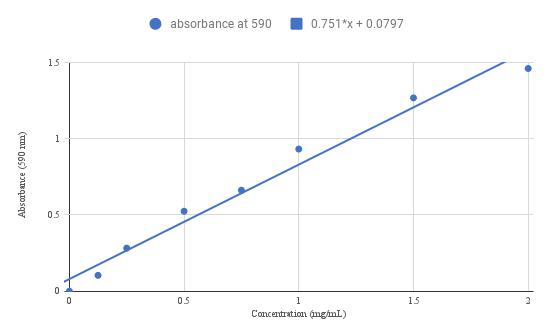
\includegraphics[width=\linewidth]{figures/bradford-standard-curve}
  \end{minipage}
  \caption{Bradford assay results. \textbf{Left:} Sample absorbance at 590 nm and extrapolated concentration. \textbf{Right:} Bradford standard curve.}
  \label{fig:bradford-assay}
\end{figure}

\subsection{References}

%%%%%%%%%%%%%%%%%%%%%%%%%%%%%%%%%%%%%%%%%%%%%%%%%%%%%%%%%%%%%%%%%%%%%
%% The same is true for Supporting Information, which should use the
%% suppinfo environment.
%%%%%%%%%%%%%%%%%%%%%%%%%%%%%%%%%%%%%%%%%%%%%%%%%%%%%%%%%%%%%%%%%%%%%
\begin{suppinfo}

\end{suppinfo}

%%%%%%%%%%%%%%%%%%%%%%%%%%%%%%%%%%%%%%%%%%%%%%%%%%%%%%%%%%%%%%%%%%%%%
%% The appropriate \bibliography command should be placed here.
%% Notice that the class file automatically sets \bibliographystyle
%% and also names the section correctly.
%%%%%%%%%%%%%%%%%%%%%%%%%%%%%%%%%%%%%%%%%%%%%%%%%%%%%%%%%%%%%%%%%%%%%
\bibliography{references}

%%%%%%%%%%%%%%%%%%%%%%%%%%%%%%%%%%%%%%%%%%%%%%%%%%%%%%%%%%%%%%%%%%%%%
%% The "tocentry" environment can be used to create an entry for the
%% graphical table of contents.
%%%%%%%%%%%%%%%%%%%%%%%%%%%%%%%%%%%%%%%%%%%%%%%%%%%%%%%%%%%%%%%%%%%%%

%% \begin{tocentry}

%% \end{tocentry}

\end{document}


results section mantra:
1 - Explain what you did and then describe what you expected as an outcome
2 - Describe the data and show the dta
3 - Interpret the data

Role of the lateral channel in catalase HPII of Escherichia coli, Loewen
They suggest that the perpendicular channel is the entrance channel and the lateral channel is the exhaust channel, because:
-enlarging the perpendicular channel increases peroxidatic activity
-perpendicular seems optimized for bringin in H2O2
-lateral channel is blocked in some catalases

Substrate Flow, Loewen
There are H2O2 binding sites in the heme distal pocket and main channel
There are several input channels; what are their purposes?
There is a ``molecular ruler'' in the main channel which selects for H2O2 against water
Active site mutations which allow more water in slow down the rxn rate
This paper discusses unidirectional flow of H2O2 through the main channel

Active and inhibited catalase structures, tainer
This is the paper about the hydrophobic ``molecular ruler''
A hydrophobic region distal to the heme cleft contains phenylalanines, tryptophan and two valines
Authors propose that two waters (one h-bonded to human Asn148 and His75; other h-bonded to gln168 and asp128) form a ``ruler''
This ``ruler'' is far enough apart that only H2O2 can stably occupy the distance betweeen, thus allowing only H2O2 to enter, not H2O
This would explain why opening the perpendicular channel decreases the rate

Site-Specific Incorporation of 3-Nitrotyrosine as a Probe of pKa Perturbation of Redox-Active Tyrosines in Ribonucleotide Reductase, Stubbe
pKa of 3NY can vary lots, between 7.5-10

\cite{kcatkm}
Km: 1.1M,
kcat/Km: 6.6*10^7/M/s

possibly make a figure with the h2o2 and water from the electric potential paper?

---------------
Arguments about protein production, validation, and ncAA validation:
We know we have wildtype protein because our gels have bands, indicating protein of the proper size was made with His tags
We know our WT protein was active by quantitative assays

We know our noncanonical protein was expressed by similar 
